\chapter{Conclusion \& Directions for a Category}\label{chap:summary}
\setlength\epigraphwidth{.7\textwidth}
\epigraph{
  but Max stepped into his private boat and waved good-bye\\
  and sailed back over a year\\
  and in and out of weeks\\
  and through a day\\
  and into the night of his very own room\\
  where he found his supper waiting for him\\
  and it was still hot.}{
  ---Maurice Sendak, \emph{Where the Wild Things Are}
}

What's the big takeaway from this project? What's the summary?

Sometimes we can reduce the behavior of objects in a messier knot
category to that of ones in a cleaner sub-category. For instance, in
studying tame knots, our motivation was to noting that all knots that
are topologically ambient isotopic to a polygonal knot inherit the
nice structure of the PL category. % As the existence of wild knots
% shows us, working in different categories can get us very different
% behavior. Hence we must always be careful to clarify the exact scope
% of our results.

However, as we saw in \cref{chap:connections-to-sn}, it seems that
broadening our perspective to the context of \np{knots that can be
  described by \emph{discrete} (but possibly infinite) packets of
  information} could be a more natural place to study tame knots. What
tools do we have for doing so? The work of \cref{chap:machinery} gave
us two key strategies: Namely, being able to separate strands from
each other (although not necessarily from themselves; that requires
the discreteness conditions), and applying uniform convergence /
bijectivity arguments to guarantee ambient isotopy under limiting
conditions.

In \cref{chap:moving-into-r3}, we used these tools to formally prove
that if we loosen the ``finite crossings'' condition on regular
diagrams to just ``discrete crossings,'' we get a formalism that is
tied to a particular class of well-behaved wild knots in a way that is
directly analogous to regular diagrams and tame knots. In particular,
regular diagrams (finite crossings) are the tools for studying
polygonal knots (finite unions of line segments), while discrete
diagrams (possibly countably many crossings) seem to offer potential
for studying ``discrete'' knots (possibly countable unions of line
segments). In a qualitative sense, this makes these ``discrete'' knots
(even the wild ones) feel much more similar to \emph{tame} knots than
to the pathological \emph{everywhere-wild} knots.

We conclude this report with a discussion of possible approaches to
making this ``qualitative'' similarity more rigorous. Our main focus
is on how we might generalize our definition of simplicial complexes
to this new context; this would represent a new category living in
between PL and TOP. Again, we would like to emphasize that this is not
the author's area of specialty (really, few things are), so we would
appreciate receiving any feedback the reader has to offer.

\section{A Countably PL Category?}
Recall the following definition for a locally-finite simplicial
complex:

\begin{definition}[Simplicial Complex]
  A \emph{simplicial complex} is a collection $K = \set{\sigma_i}$
  of linear simplices such that:
  \begin{enumerate}
    \item For all $\sigma \in K$, if $\tau$ is a face of $\sigma$,
      then $\tau \in K$.
    \item For all $\sigma_1, \sigma_2 \in K$, if $\tau = \sigma_1
      \cap \sigma_2 \neq \varnothing$, then $\tau$ is a face of both
      $\sigma_1$ and $\sigma_2$. \qedhere
  \end{enumerate}
\end{definition}
We also have
\begin{definition}
  Let $K$ be a simplicial complex. Then we define the
  \emph{underlying space} of $K$ (denoted $\abs{K}$) by
  \[
    \abs{K} = \bigcup_{\sigma \in K} \sigma. \qedhere
  \]
\end{definition}
\begin{example}
  Consider the following simplicial complex:
  \begin{figure}[H]
    \centering
    \begin{tikzpicture}[scale=1.5]

      \coordinate (t) at (0,1);
      \coordinate (l) at (-1, 0);
      \coordinate (r) at (1,0);
      \coordinate (b) at (0,-1);
      \coordinate (c) at (0,0);
      \fill[red!20!white, opacity=.5] (t) -- (l) -- (c) -- (t) (r)
      -- (c) -- (b) -- (r);

      \begin{scope}[every node/.style={draw, circle, inner sep=1pt,
          fill=white}]
        \node (t) at (t) {};
        \node (r) at (r) {};
        \node (l) at (l) {};
        \node (b) at (b) {};
        \node (c) at (c) {};
      \end{scope}


      \node[above, yshift=2pt] () at (t) {$t$};
      \node[right, xshift=3pt] () at (r) {$r$};
      \node[left, xshift=-3pt] () at (l) {$\ell$};
      \node[below, yshift=-2pt] () at (b) {$b$};
      \node[above right] () at (c) {$c$};

      \draw (t) -- (l) -- (b) -- (r) -- (t) (t) -- (c) -- (b) (l) --
      (c) -- (r);
    \end{tikzpicture}
  \end{figure}
  The simplices are as follows (Note, we'll use $\ip{v_1, v_2,
    \ldots, v_n}$ to denote ``the convex hull of $\set{v_1, v_2,
    \ldots, v_n}$'').
  \begin{enumerate}
    \item The 0-simplices: $K^0 = \set{\ip{t}, \ip{\ell}, \ip{b},
      \ip{r}, \ip{c}}$
    \item The 1-simplices: $K^1 = \set{\ip{t,\ell}, \ip{\ell, b},
      \ip{b, r},
      \ip{r, t}, \ip{t,c}, \ip{\ell, c}, \ip{b,c}, \ip{r,c}}$
    \item The 2-simplices: $K^2 = \set{\ip{t,\ell,c},
      \ip{b,r,c}}$.
  \end{enumerate}
  One can verify the axioms are satisfied. The underlying space is
  just all of the stuff except for the interior of the two white
  simplices, $\ip{t,r,c}$ and $\ip{b,\ell, c}$.
\end{example}
Now another definition.
\begin{definition}[Locally finite]
  Let $K$ be a simplicial complex. Then we say $K$ is
  \emph{locally finite} if for all 0-simplices $\sigma \in K$,
  $\sigma$ is a vertex of only finitely-many simplices of $K$.
\end{definition}
If one is not careful, this definition for locally-finite can create
some unexpected collections being referred to as ``simplicial
complexes.'' Of course, the weak topology is meant to prevent
silly situations such as these, but we'll pretend it doesn't exist for
the time being. This allows us to construct some PL-flavored
structures that seem germane to examining wild knots in a way that's
agnostic to the pathology at the wild point.
\begin{example}\label{ex:locally-finite-problem}
  Consider a proposed simplicial complex defined as follows.
  \begin{leftbar}
    \begin{enumerate}
      \item For all $n \in \NN$, let $I_n$ be defined by
        \[
        I_n = \bk{\frac{1}{2^n},\ \frac{1}{2^{n-1}}}
        \]
        Observe these are all $1$-simplices.
      \item Also define
        \[
        a_n = \set{\frac{1}{2^n}} \qquad\qquad\qquad\qquad b_n =
        \set{\frac{1}{2^{n-1}}}
        \]
        and
        \[
        I_\infty = \set{0}.
        \]
        Observe these are all $0$-simplices. Also note that $\partial
        I_n = a_n \cup b_n$.
    \end{enumerate}
    Let $S = I_\infty \cup \bigcup_{n \in \NN} \set{I_n, a_n, b_n}$
    (just scooping up all the items defined above). Is this a valid
    simplicial complex? Is it locally finite? \qedhere
  \end{leftbar}
\end{example}
\begin{sproof}[Sketch]
  We break the statement into parts. The results are straightforward,
  we have just sought to be exhaustive for completeness.
  \begin{leftbar}
    \textbf{Claim 1:} The collection $S$ defined in the question is a
    valid simplicial complex.

    \noindent \textbf{Proof of Claim 1:}
    \begin{enumerate}
      \item First, we verify that for all $\sigma \in K$, if $\tau$ is
        a face of $\sigma$, then $\tau \in K$.

        Let $\sigma \in K$ be arbitrary. We have two sub-cases.
        \begin{enumerate}[label=\arabic*)]
          \item Suppose $\sigma$ is a 0-simplex. Then $\sigma$ is its
            only face, so the claim holds.
          \item Suppose $\sigma$ is a 1-simplex. Then by construction,
            there exists $n \in \NN$ such that $\sigma =
            \bk{\frac{1}{2^n}, \frac{1}{2^{n-1}}}$. Hence the faces of
            $\sigma$ are $a_n = \set{\frac{1}{2^n}}$ and $b_n =
            \set{\frac{1}{2^{n-1}}}$, both of which are elements of $S$
            (by construction).
        \end{enumerate}
        Hence we see that the first condition is satisfied.
      \item Let $\sigma_1, \sigma_2 \in K$ be arbitrarily chosen. We
        want to show that if $\tau = \sigma_1 \cap \sigma_2 \neq
        \varnothing$, then $\tau$ is a face of both $\sigma_1$ and
        $\sigma_2$.

        First, note that if $\sigma_1 = \sigma_2$, then the claim is
        trivial. Hence suppose $\sigma_1 \neq \sigma_2$. We proceed by
        casework.
        \begin{enumerate}[label=\arabic*)]
          \item Suppose $\sigma_1$, $\sigma_2$ are both 0-simplices.
            Then since $\sigma_1 \neq \sigma_2$, we have $\sigma_1
            \cap \sigma_2 = \varnothing$, so the claim is satisfied
            vacuously.
          \item Now suppose one of $\sigma_1, \sigma_2$ is $I_\infty$.
            Note that for any $n \geq 0$, $I_\infty$ is disjoint from
            \emph{each} of $a_n$, $b_n$, and $I_n$. Hence $\sigma_1 \cap
            \sigma_2 = \varnothing$, so in this case the claim is also
            satisfied vacuously.
          \item Now suppose at least one of $\sigma_1, \sigma_2$ is not
            a 0-simplex, and that neither $\sigma_1, \sigma_2$ is
            $I_\infty$.\footnote{This is wordy, but we're just taking
            the complement of the two cases we've already done.} One can
            verify the following:
            \begin{enumerate}[label=\roman*)]
              \item Suppose one of $\sigma_1$, $\sigma_2$ is a 0-simplex
                and the other is a 1-simplex. Without loss of
                generality, let $\sigma_1$ be the 1-simplex and
                $\sigma_2$ be the 0-simplex. Then $\sigma_1$ is of the
                form $I_n = \bk{\frac{1}{2^n},\ \frac{1}{2^{n-1}}} =
                \ip{a_n \cup b_n}$ for some $n$ (recall, $a_n$, $b_n$
                were defined as 1-element sets). Then $\sigma_1 \cap
                \sigma_2 \neq\varnothing$ iff $\sigma_2$ is one of
                $a_n$ or $b_n$, at which point the claim follows by
                construction of $S$.
              \item Suppose $\sigma_1$, $\sigma_2$ are of the form $I_n$,
                $I_m$ respectively, and without loss of generality,
                suppose $n > m$. Then observe we have $I_n \cap I_m
                \neq \varnothing$ iff $n = m+1$. In this case, we see
                $I_n \cap I_m = \set{\frac{1}{2^{n-1}}} =
                \set{\frac{1}{2^m}}$, which is an element of $S$ by
                construction.
            \end{enumerate}
        \end{enumerate}
        In any case, we see the condition is satisfied.
    \end{enumerate}
    It follows that $S$ is a valid simplicial complex.
  \end{leftbar}

  \begin{leftbar}
    \textbf{Claim 2:} $S$ is locally finite.

    \noindent \textbf{Proof of Claim:} By a similar argument to the
    above, one can verify that
    \begin{enumerate}
      \item For all $n \in \NN$, we have $I_\infty \cap a_n = I_\infty
        \cap b_n = I_\infty \cap I_n$. Hence $I_\infty$ is a vertex of
        exactly one simplex, namely itself.
      \item For all $n \in \NN$, $a_n$ is a vertex of $I_n$ and
        $I_{n+1}$. Similarly, for $n > 2$, $b_n$ is a vertex of
        $I_{n-1}$, $I_n$. For $n = 1$, $b_1$ is a vertex of $I_1$ and
        that's it.
    \end{enumerate}
    In any case, we see that the simplicial complex is locally finite.
  \end{leftbar}

  \begin{leftbar}
    \textbf{Claim 3:} $\abs{S} = [0,1]$.

    \noindent \textbf{Proof of Claim 3:} Let $x \in [0,1]$ be
    arbitrary. We want to show $\exists \sigma \in K$ such that $x \in
    \sigma$. We proceed by casework.
    \begin{enumerate}
      \item Suppose $x = 0$. Then $x \in I_\infty$, as desired.
      \item Suppose that $x \neq 0$. Then there exists $n \in \NN$ such
        that
        \[
        \frac{1}{2^{n}} \leq x \leq \frac{1}{2^{n-1}},
        \]
        from which we have $x \in I_n$.\footnote{
        To be extremely explicit: one can take $\log_2$ of each term in
        the inequality above; since $\log_2$ is monotonic, the
        ordering is preserved. Then, one can use the Archimedean
        property of the reals to obtain the existence of the desired
        $n$.}
    \end{enumerate}
    In either case, it follows that there exists $\sigma \in K$ such
    that $x \in \sigma$. Hence $[0,1] \subseteq \bigcup_{\sigma \in K}
    \sigma$. Now observe that by construction, for all $\sigma \in K$,
    $\sigma \subseteq [0,1]$. Hence $\bigcup_{\sigma \in K} \sigma =
    [0,1]$.

    Hence we have $\abs{S} = [0,1]$, as desired.
  \end{leftbar}
  In any case, we see that according to all of our definitions, this
  is a honest-to-goodness locally-finite simplicial complex.
\end{sproof}
As we mentioned way back in \cref{chap:intro}, one can construct
similar simplicial complexes in $\RR^n$. For instance, consider the
following collection in $\RR^2$:
\begin{figure}[H]
  \centering
  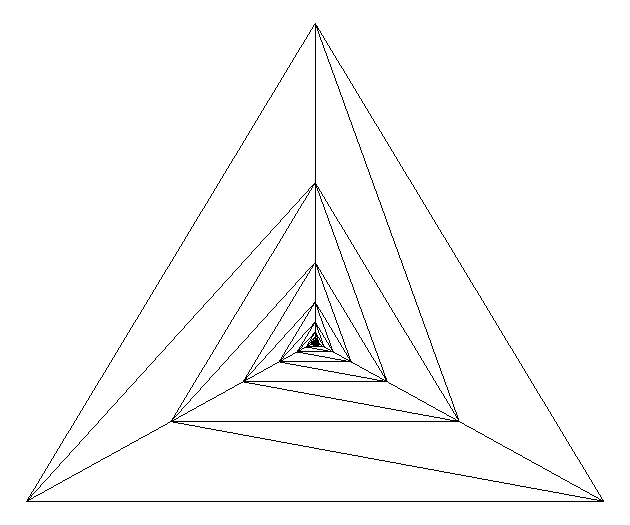
\includegraphics[scale=.5]{figures/wild/simp-comp-down.pdf}
  \caption{A ``locally-finite'' simplicial complex.}
\end{figure}
Analogous objects in $\RR^3$ seem like they could be very apt for
describing ``discrete'' wild knots, especially in light of
\cref{thm:discrete-diagram-countably-polygonal}. Of course, we must be
careful not to go \emph{too} far in this direction; for instance, we
would not want to include objects like the following:
\begin{example}[Non-example]
  Let $K = \set{\sigma_i}$ be a collection of linear simplices defined
  by
  \[
    K = \set{\set{x} \MID x \in \RR}. \qedhere
  \]
\end{example}
This particular behavior could be constrained by requiring that $K$ be
countable, but that would still allow for complexes like the
following:
\begin{example}[Non-example]
  Let $K = \set{\sigma_i}$ be a collection of linear simplices defined
  by
  \[
    K = \set{\set{x} \MID x \in \QQ}. \qedhere
  \]
\end{example}
Inspired by these examples (but also by wanting to prevent the
non-examples given above), we imagine we could achieve the desired
effects by looking at something like the following (note, we encourage
the reader to improve upon our naming conventions):
\begin{definition}[A proposed definition]
  Let $K = \set{\sigma_i}$ be a simplicial complex. Define $K$ to be
  \emph{almost locally finite} if it is locally finite at all but
  finitely-many $0$-simplices.
\end{definition}
Or maybe something like the following:
\begin{definition}[Another proposed definition]
  Let $K = \set{\sigma_i}$ be a locally-finite simplicial complex.
  Define a \emph{feral point} of $K$ to be a $0$-simplex $\triangle^0
  \in K$ such that for all $\varepsilon > 0$, there exists
  infinitely-many $\sigma_i \in K$ such that
  $B_\varepsilon(\triangle^0) \cap \sigma_i \neq \varnothing$. Then
  endow $K$ with the subspace topology, and call $K$
  \emph{countably-PL} if there are only finitely-many feral points.
\end{definition}
We'd be interested in seeing if any of these proposed definitions
provide us \emph{objects} for a new category. Morphisms would be
similar to PL maps, only now with extra requirements to respect the
``feral'' structure, e.g.\ feral points map to feral points, plus
maybe some analogue to the star condition at these points.

We hope that future work in this direction might help to shed light on
deeper structure to knots. We are particularly excited about the
implications of \cref{chap:connections-to-sn}, and wonder whether they
can be generalized to \emph{everywhere-wild} knots. In particular, to
study these ``discrete'' knots we used symmetry groups of discrete
sets. We wonder whether continuous symmetry groups could be used to
study wild knots, which (in some sense) have ``continuous''
collections of crossings (although it seems we lose transverseness).

We'd also be interested in seeing deeper study of feral points,
particularly diagrammatic invariants for distinguishing them from wild
points. Lastly, we'd like to see a careful proof of an analogue to
Reidemeister's theorem in this new context, as well the development of
a new, slightly-stronger category in which to study our embeddings.



% naturally suited to studying well-behaved wild knots


% To the best of our knowledge, not many
% --- the question hasn't really been broached before. Our goal for this
% section is to very briefly remind the reader of some of the properties
% of our three categories, and point out ways in which PL could be
% extended to include some moderately well-behaved wild knots.

% {\color{blue} Just some short blurb here will suffice!}

%%% Local Variables:
%%% TeX-master: "../../kobayashi-thesis"
%%% End:
